\chapter{Spring Data JPA}

\fcolorbox{black}[HTML]{E9F0E9}{\parbox{\textwidth}{%
\noindent \textbf{Learning goals}\\
De junior-collega
\begin{enumerate}[nolistsep]
\item kan het concept ORM beschrijven.
\item kan uitleggen wat JPA is.
\item kan verschillende JPA-implementaties benoemen.
\item kan beschrijven wat een \textit{persistence unit} is.
\item kan de fundamentele interfaces van JPA beschrijven.
\item kan uitleggen wat de \textit{persistence context} is.
\item kan entiteitsklassen implementeren.
\item kan de levenscyclus van entiteitsobjecten beschrijven.
\item kan verschillende soorten relaties tussen entiteitsklassen implementeren.
\item kan CRUD-operaties implementeren.
\item kan query's implementeren.
\end{enumerate}
}}

  
\section{Wat is ORM?}

Object-Relational Mapping (ORM) is een techniek waarmee je gegevens uit een relationele database kunt opvragen en manipuleren met behulp van een objectgeoriënteerde programmeertaal.

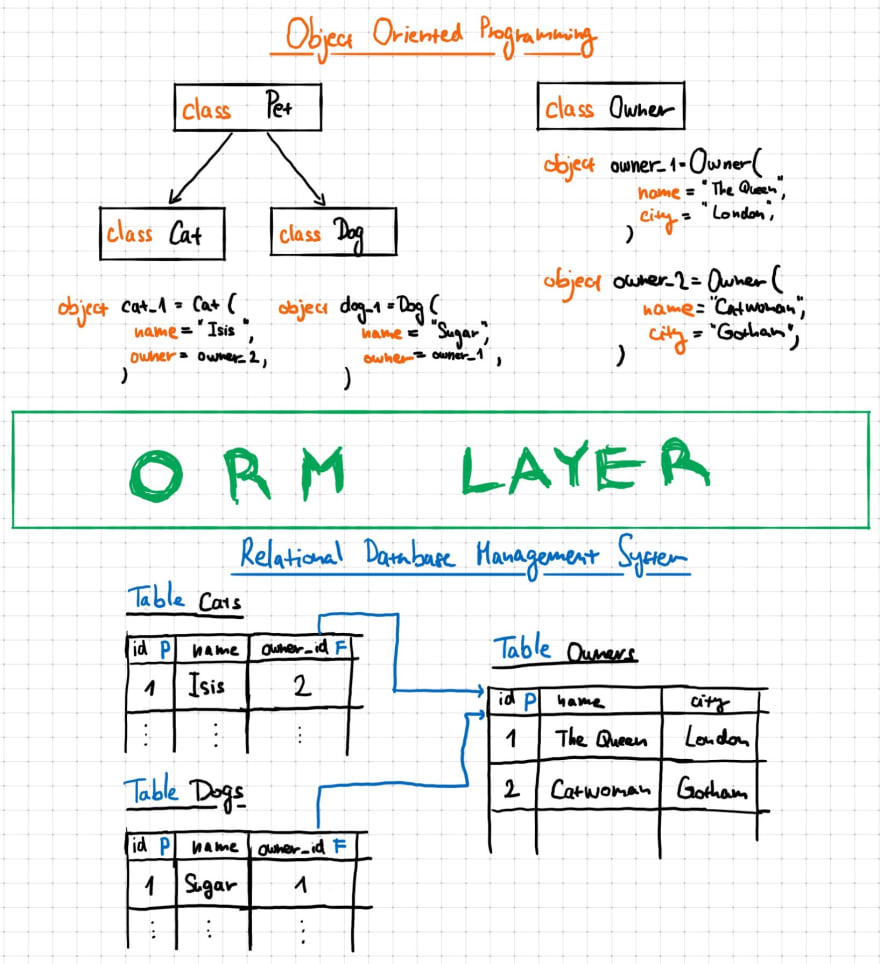
\includegraphics[width=\textwidth]{./images/chapter6/orm}


\section{Wat is JPA?}

De Java Persistence API (officieel hernoemd naar Jakarta Persistence API) is een specificatie die definieert hoe gegevens gepersisteerd kunnen worden in een Java-toepassing. 

JPA is een specificatie. Dit betekent dat JPA bestaat uit implementatie richtlijnen voor de Java ORM-laag. De specificatie wordt alleen geleverd met interfaces, zonder eigenlijke implementatie.  Er wordt een referentie-implementatie voorzien, maar andere bedrijven kunnen hun eigen implementatie van de specificatie maken en distribueren.


\frame{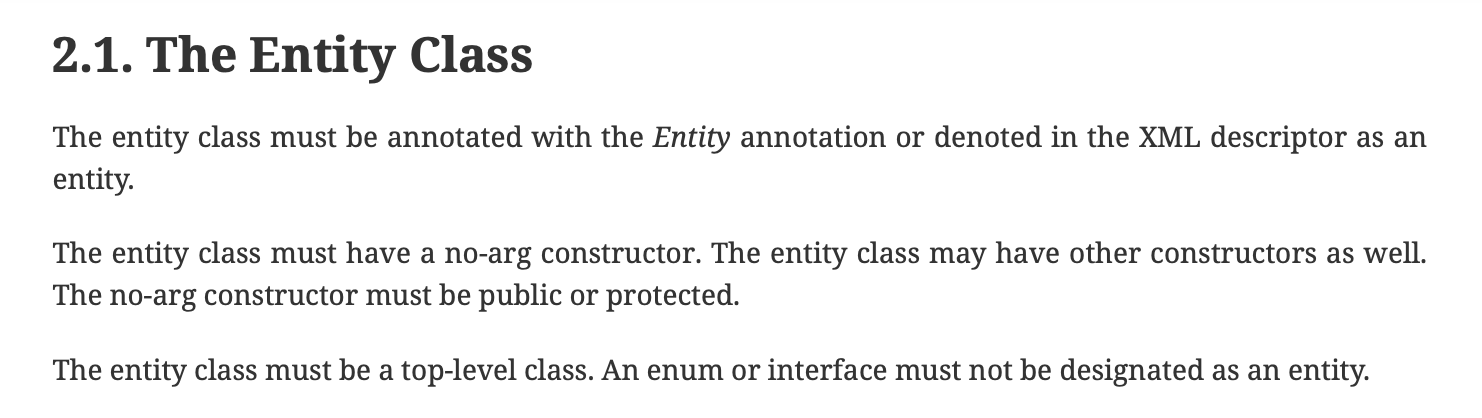
\includegraphics[width=\textwidth]{./images/chapter6/entity_class_specification}}

In deze cursus gebruiken we Hibernate als implementatie van de JPA specificatie \footnote{\url{https://hibernate.org/ and https://hibernate.org/orm/}}.  

Spring Data JPA biedt extra functionaliteit en vereenvoudigt het werken met JPA. 
Je krijgt een no-code implementatie van het repository design pattern. Database query's kunnen gegenereerd worden  door Spring Data JPA aan de hand van een methodenaam.


\section{Datasource}

De datasource of gegevensbron is de configuratie die wordt gebruikt om verbinding te maken met een database of andere externe gegevensopslag. Het bevat informatie  zoals de database-URL, gebruikersnaam, wachtwoord en andere instellingen die nodig zijn om gegevens uit een externe bron op te halen of ernaar te schrijven.

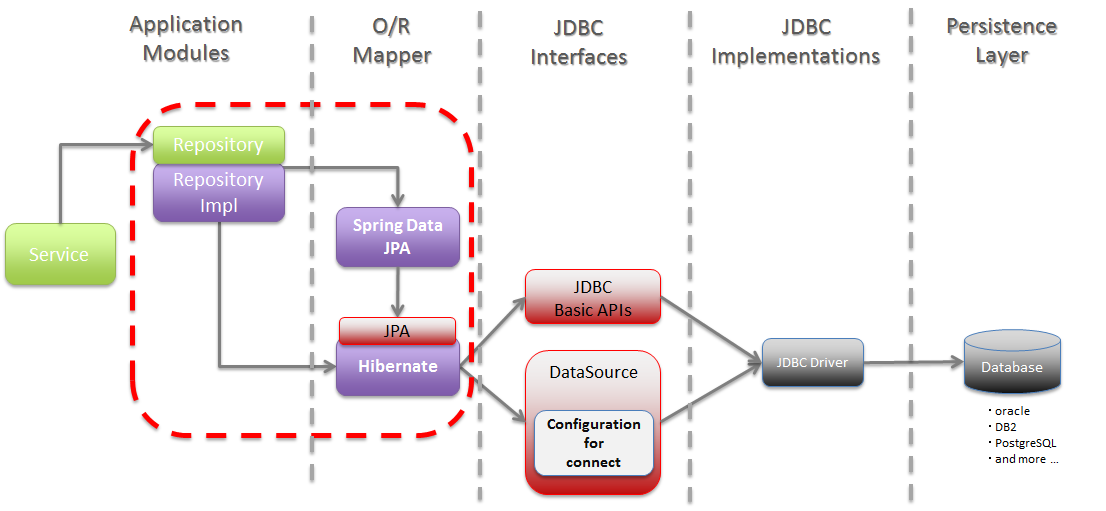
\includegraphics[width=\textwidth]{./images/chapter-jpa/springdatajpa}

De datasource wordt gespecificeerd in het bestand \textit{application.properties}.
Volgende eigenschappen kun hier hiervoor gebruiken:

\begin{tabular}{|l|p{8cm}|}
\hline
spring.datasource.url & JDBC URL van de database.\\
spring.datasource.username & Gebruikersnaam voor de database.\\
spring.datasource.password & Paswoord voor de database.\\
spring.jpa.show-sql & Logging van de SQL statements. Default: false\\
spring.jpa.hibernate.ddl-auto & Automatisch genereren van tabellen. Mogelijke waarden: none (production), create, create-drop, validate and update. \footnote{\url{https://stackoverflow.com/questions/42135114/how-does-spring-jpa-hibernate-ddl-auto-property-exactly-work-in-spring}}\\
\hline
\end{tabular}

De H2 in-memory databank die we in het vorige hoofdstuk hebben gebruikt, gaan we nu vervangen door een MySQL databank. 
We zullen de MySQL-database draaien in een Docker-container.  Elke databaseserver heeft zijn eigen specifieke protocol voor de overdracht van gegevens tussen de server en  het programma.  Vergeet niet om de h2-dependency in de pom.xml te vervangen door de MySQL-driver.

\begin{lstlisting}
<dependency>
      <groupId>com.mysql</groupId>
      <artifactId>mysql-connector-j</artifactId>
      <scope>runtime</scope>
</dependency>
\end{lstlisting}

De volgende docker-compose.yml kan gebruikt worden om een docker-container met een MySQL databaseserver te starten. 
Ga naar de folder waar dit bestand opgeslagen is en voer het commando \verb|docker compose up| uit.

\begin{lstlisting}
version: "3.3"

services:
  superhero-db:
    image: mysql:latest
    ports:
      - "3306:3306"
    environment:
      MYSQL_DATABASE: 'superherodb'
      MYSQL_USER: 'user'
      MYSQL_PASSWORD: 'password'
      MYSQL_ROOT_PASSWORD: 'admin'
\end{lstlisting}

\begin{oefening}
Zorg dat je superhero-backend project gebruik maakt van een MySQL databank. 
Pas de nodige dependencies in de pom.xml aan. Maak de folder \textit{src/main/docker} aan en voeg hier het bestand docker-compose.yml toe. 
Start de MySQL database server op. Voeg de volgende configuratie toe in het bestand \textit{application.properties}:

\begin{lstlisting}
spring.datasource.url=jdbc:mysql://localhost:3306/superherodb
spring.datasource.username=user
spring.datasource.password=password
spring.jpa.hibernate.ddl-auto=update
\end{lstlisting}

Start de Spring Boot applicatie. 
\end{oefening}

IntellliJ IDEA heeft een database-tool waarmee je de database kan inspecteren. Deze tool werkt niet voor een h2 database, dan gebruik je de h2-console.

\frame{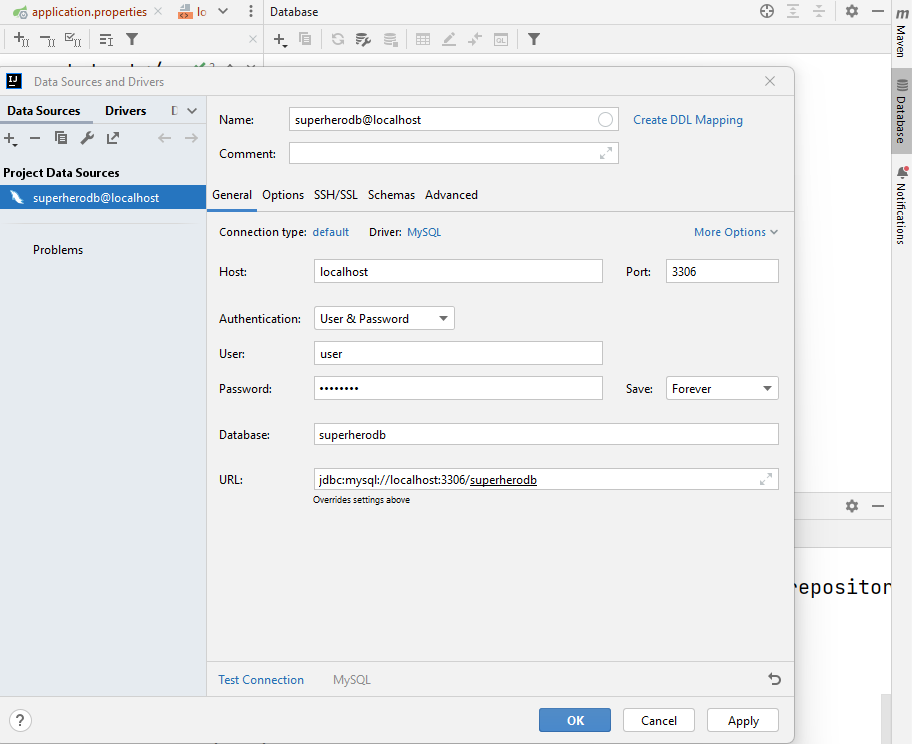
\includegraphics[width=\textwidth]{./images/chapter-jpa/datasource_intellij}}

\frame{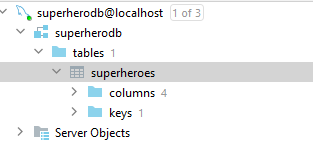
\includegraphics{./images/chapter-jpa/superherodb_localhost}}

De eigenschap \textit{spring.jpa.hibernate.ddl-auto} bepaalt hoe Hibernate omgaat met het genereren van het databaseschema. 
De volgende waarden zijn mogelijk voor deze eigenschap:

\begin{tabular}{|l|p{8cm}|}
\hline
none & Hibernate voert geen schemageneratie of validatie uit.\\
validate & Hibernate valideert het bestaande schema ten opzichte van de entiteitsklassen en meldt eventuele verschillen zonder het schema te wijzigen.\\
update & Hibernate werkt het bestaande schema bij op basis van de entiteitsklassen. Het voegt tabellen, kolommen of beperkingen toe voor nieuwe entiteiten of wijzigingen aan bestaande entiteiten. Het laat bestaande tabellen of kolommen ongemoeid.\\
create & Hibernate maakt het schema vanaf nul, waarbij tabellen worden verwijderd en opnieuw gemaakt, wat kan leiden tot gegevensverlies.\\
create-drop & Vergelijkbaar met create, maar het schema wordt verwijderd wanneer de SessionFactory wordt gesloten (bijvoorbeeld wanneer de toepassing wordt afgesloten).\\
\end{tabular}

De eigenschappen create en update kunnen handig zijn tijdens de ontwikkeling, wanneer je wilt dat Hibernate het schema automatisch genereert. 

In een productieomgeving wordt aanbevolen om automatische schemageneratie uit te schakelen (none) of,  op zijn minst,  alleen validatie uit te voeren (validate) zonder het schema te wijzigen. Het is ook belangrijk om versiebeheer voor het databaseschema te hebben. Hiervoor gebruik je migratietools zoals Flyway of Liquibase.

\section{De Entity klasse}

\begin{lstlisting}[frame=single,language=java]
package be.pxl.superhero.domain;

import jakarta.persistence.*;
import org.apache.logging.log4j.LogManager;
import org.apache.logging.log4j.Logger;

import java.util.ArrayList;
import java.util.List;

@Entity
@Table(name="superheroes")
public class Superhero {

	private static final Logger LOGGER = LogManager.getLogger(Superhero.class);

	@Id
	@GeneratedValue(strategy = GenerationType.IDENTITY)
	private Long id;
	
	private String firstName;
	private String lastName;
	@Column(unique = true)
	private String superheroName;
	@Column(name="notes")
	private String description;

	public Superhero() {
		// JPA only
	}

	public Superhero(String firstName, String lastName, String superheroName) {
		if (LOGGER.isDebugEnabled()) {
			LOGGER.debug("Creating a new superhero...");
		}
		this.firstName = firstName;
		this.lastName = lastName;
		this.superheroName = superheroName;
	}

	public Long getId() {
		return id;
	}

	public String getFirstName() {
		if (LOGGER.isTraceEnabled()) {
			LOGGER.trace(String.format("FirstName of %s was revealed.", superheroName));
		}
		return firstName;
	}

	public void setFirstName(String firstName) {
		this.firstName = firstName;
	}

	public String getLastName() {
		if (LOGGER.isFatalEnabled()) {
			LOGGER.fatal(String.format("LastName of %s was revealed.", superheroName));
		}
		return lastName;
	}

	public void setLastName(String lastName) {
		this.lastName = lastName;
	}

	public String getSuperheroName() {
		return superheroName;
	}

	public void setSuperheroName(String superheroName) {
		this.superheroName = superheroName;
	}

	@Override
	public String toString() {
		return superheroName;
	}
}
\end{lstlisting}

Een JPA-entityklasse is een POJO (Plain Old Java Object) klasse gebruikt wordt om objecten in de database te vertegenwoordigen.

De \textbf{@Id}-annotatie duidt de primaire sleutel aan.

De \textbf{@Column}-annotatie wordt gebruikt om details van de kolom te specificeren. 
Met de @Column-annotatie kan je de volgende attributen aanpassen:
\begin{itemize}
\item \textbf{name}: specificeer de naam van de kolom.
\item \textbf{length}: specificeer de grootte van de kolom, met name voor een String-waarde.
\item \textbf{nullable}: markeer de kolom als NOT NULL wanneer het databaseschema wordt gegenereerd.
\item \textbf{unique}:  de kolom om alleen unieke waarden te bevatten.
\end{itemize}


\begin{oefening}
$\square$ Maak een entity-klasse Mission.
Een missie heeft de volgende velden:
\begin{tabular}{|c|c|c|}
\hline
id & Long & De primaire sleutel.\\
name & String & Unieke naam van de missie.\\
completed & boolean & De missie is voltooid.\\
\hline
\end{tabular}
\end{oefening}

\section{Repository}

De JpaRepository-interface is een uitbreiding van CrudRepository.
JpaRepository breidt PagingAndSortingRepository uit, dat op zijn beurt CrudRepository uitbreidt.

Hun belangrijkste functies zijn:

\begin{itemize}
\item CrudRepository biedt voornamelijk CRUD-functies.
\item PagingAndSortingRepository biedt methoden voor paginering en het sorteren van records.
\item JpaRepository biedt enkele JPA-gerelateerde methoden, zoals het flushen van de persistentiecontext en het verwijderen van records in batches.
\end{itemize}

\begin{oefening}
Maak de interface MissionRepository aan. Maak daarna de MissionService en MissionController zodat het mogelijk wordt om een missies aan te maken, op te halen (zowel adhv id als een volledige lijst), te updaten en te verwijderen.  Voeg de nodige DTOs toe. Hou er rekening mee dat de namen van missies uniek moeten zijn. Voorzie je eigen exceptions en zorg voor de nodige foutafhandeling.

\frame{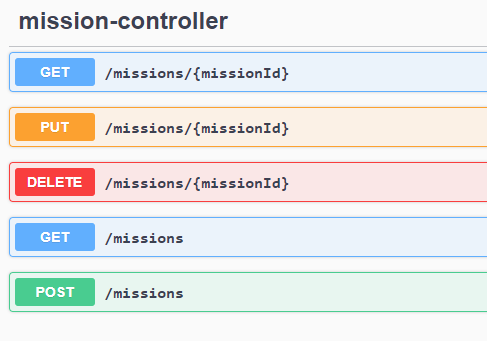
\includegraphics[width=\textwidth]{./images/chapter-jpa/mission_controller}}

\frame{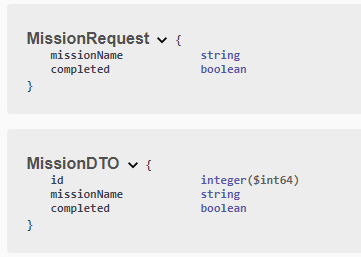
\includegraphics{./images/chapter-jpa/mission_api}}
\end{oefening}


\section{Entity lifecycle}


De PersistenceContext is \'e\'en van de belangrijkste concepten in JPA. Het is de verzameling van alle entiteitsobjecten die momenteel gebruikt worden of recentelijk zijn gebruikt. Je kunt de PersistenceContext beschouwen als een soort first-level cache. Elk entiteitsobject in de PersistenceContext vertegenwoordigt een record in de database. De PersistenceContext beheert deze entiteitsobjecten en hun levenscyclus. Elk entiteitsobject heeft \'e\'en van de 4 statussen: New,  Managed, Removed en Detached.


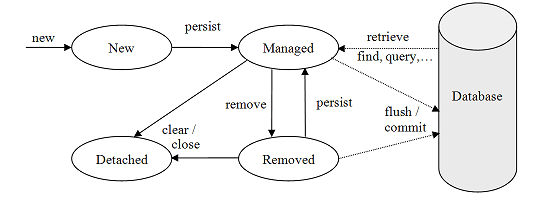
\includegraphics[width=\textwidth]{./images/chapter6/entity_states}

Een nieuw aangemaakt entiteitsobject bevindt zich in status \textbf{New} . Het entiteitsobject is nog niet opgeslagen, dus er is nog geen database-record. Het De PersistenceContext is nog niet op de hoogte van het bestaan van het entiteitsobject.

Alle entiteitsobjecten die aan de PersistenceContext zijn gekoppeld, bevinden zich in de status \textbf{Managed}. Een entiteitsobject wordt beheerd wanneer het wordt opgeslagen in de database. Entiteitsobjecten die uit de database worden opgehaald, bevinden zich ook in de status \textbf{Managed}.  Als een beheerd entiteitsobject wordt aangepast binnen een actieve transactie,  dan detecteert de PersistenceContext de wijziging en wordt deze doorgegeven aan de database.

Wanneer een beheerd entiteitsobject binnen een actieve transactie wordt verwijderd, verandert de status van beheerd naar verwijderd, en wordt het record fysiek uit de database verwijderd (wanneer de transactie wordt bevestigd).

Een entiteit wordt losgekoppeld (detached) wanneer deze niet langer wordt beheerd door de PersistenceContext maar nog steeds een record in de database vertegenwoordigt. Losgekoppelde entiteitsobjecten hebben beperkte functionaliteit.

Bij het gebruik van Spring Data JPA hoeven we zelf geen interactie met de entitymanager te implementeren. Wanneer een Repository wordt aangemaakt, biedt de door Spring Data JPA geleverde SimpleJpaRepository-klasse de standaardimplementatie. De SimpleJpaRepository-klasse gebruikt intern de JPA-entitymanager.

\begin{oefening}
Bestudeer de klasse  SimpleJpaRepository (bijv. save()-methode).
\end{oefening}


\section{Query's}

Met Spring Data JPA kun je query-methoden cre\"eren om records uit de database te selecteren zonder SQL-query's te schrijven. Achter de schermen zal Spring Data JPA SQL-query's genereren op basis van de query-methode en de query vervolgens uitvoeren.

Spring Data JPA kan de query afleiden uit de naam van de query-methode.

In een UserRepository kan je bijvoorbeeld een query-methode hebben met de naam findByEmailAddressAndLastname().

\begin{lstlisting}
public interface UserRepository extends JpaRepository<User, Long> {
  List<User> findByEmailAddressAndLastname(String emailAddress, String lastname);
}
\end{lstlisting}

Spring Data JPA genereert achter de schermen een query die wordt vertaald naar de JPQL-query: select u from User u where u.emailAddress = ?1 and u.lastname = ?2.

\begin{oefening}
Voeg in de interface SuperheroRepository een methode toe om een Superhero terug te vinden aan de hand van zijn superheldennaam. De methode retourneert een Optional.
\end{oefening}


\section{Relationships}
Vanuit een databaseperspectief hebben we de volgende relaties tussen tabellen:
\begin{itemize}
\item one-to-many
\item one-to-one
\item many-to-many
\end{itemize}

JPA biedt meerdere annotaties aan om deze relaties in de code te weerspiegelen.  Voor de superhero-backend gebruiken we een many-to-many relatie tussen superhelden en missies. Een superheld kan deelnemen aan meerdere missies, en meerdere superhelden bundelen hun krachten in één missie. Een koppelingstabel is noodzakelijk om deze gegevens op te slaan.

Relaties kunnen zowel unidirectioneel als bidirectioneel zijn. Slechts één partij in een relatie is de eigenaar van de relatie.


\subsection{Many-to-many bidirectional relationship}

De Superhero-klasse is de eigenaar van de relatie tussen Mission en Superhero. Omdat de relatie bidirectioneel is, onderhouden we altijd een set van de missies van een superheld en in een missie onderhouden we een set van de deelnemende superhelden.
Wanneer je een missie aan een superheld toevoegt, moet je ervoor zorgen dat de superheld ook wordt toegevoegd aan de lijst van superhelden van de missie.
Bestudeer onderstaande code.


\begin{lstlisting}
package be.pxl.superhero.domain;

import jakarta.persistence.*;
import org.apache.logging.log4j.LogManager;
import org.apache.logging.log4j.Logger;

import java.util.ArrayList;
import java.util.List;

@Entity
@Table(name="superheroes")
public class Superhero {

	private static final Logger LOGGER = LogManager.getLogger(Superhero.class);

	@Id
	@GeneratedValue(strategy = GenerationType.IDENTITY)
	private Long id;
	
	private String firstName;
	private String lastName;
	@Column(unique = true)
	private String superheroName;
	@Column(name="notes")
	private String description;
	@ManyToMany
	private List<Mission> missions = new ArrayList<>();

	public Superhero() {
		// JPA only
	}

	public Superhero(String firstName, String lastName, String superheroName) {
		if (LOGGER.isDebugEnabled()) {
			LOGGER.debug("Creating a new superhero...");
		}
		this.firstName = firstName;
		this.lastName = lastName;
		this.superheroName = superheroName;
	}

	public Long getId() {
		return id;
	}

	public String getFirstName() {
		if (LOGGER.isTraceEnabled()) {
			LOGGER.trace(String.format("FirstName of %s was revealed.", superheroName));
		}
		return firstName;
	}

	public void setFirstName(String firstName) {
		this.firstName = firstName;
	}

	public String getLastName() {
		if (LOGGER.isFatalEnabled()) {
			LOGGER.fatal(String.format("LastName of %s was revealed.", superheroName));
		}
		return lastName;
	}

	public void addMission(Mission mission) {
		if (mission.isCompleted()) {
			throw new IllegalArgumentException("This mission was already completed.");
		}
		if (onMission(mission)) {
			throw new IllegalArgumentException("This mission was already assigned.");
		}
		missions.add(mission);
		mission.addSuperhero(this);
	}

	public boolean onMission(Mission mission) {
		return missions.stream().anyMatch(m -> m.getName().equals(mission.getName()));
	}

	public List<Mission> getMissions() {
		return missions;
	}

	public void setLastName(String lastName) {
		this.lastName = lastName;
	}

	public String getSuperheroName() {
		return superheroName;
	}

	public void setSuperheroName(String superheroName) {
		this.superheroName = superheroName;
	}

	@Override
	public String toString() {
		return superheroName;
	}
}
\end{lstlisting}

\begin{lstlisting}
package be.pxl.superhero.domain;

import jakarta.persistence.*;

import java.util.ArrayList;
import java.util.List;

@Entity
public class Mission {
	@Id
	@GeneratedValue(strategy = GenerationType.IDENTITY)
	private Long id;

	@Column(unique = true)
	private String name;

	private boolean completed;

	@ManyToMany(mappedBy = "missions")
	private List<Superhero> superheroes = new ArrayList<>();

	public Long getId() {
		return id;
	}

	public String getName() {
		return name;
	}

	public void setName(String name) {
		this.name = name;
	}

	public boolean isCompleted() {
		return completed;
	}

	public void setCompleted(boolean completed) {
		this.completed = completed;
	}

	public void addSuperhero(Superhero superhero) {
		superheroes.add(superhero);
	}

	public List<Superhero> getSuperheroes() {
		return superheroes;
	}


}
\end{lstlisting}


\begin{oefening}
Voeg de bi-directionele many-to-many relatie toe tussen de entity-klasse SuperHero en Mission.
\end{oefening}

\section{Transactions}

Nu kunnen we superhelden laten deelnemen aan een missie.

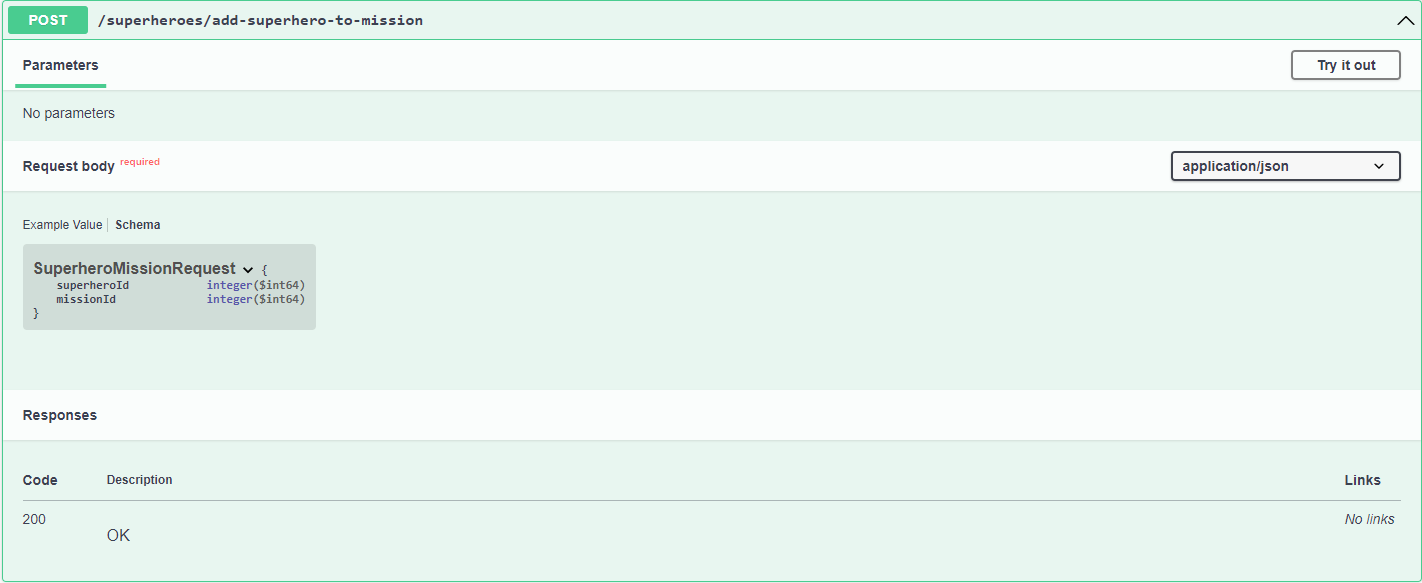
\includegraphics[width=\textwidth]{./images/chapter-jpa/superhero_controller_add_superhero_to_mission}

\begin{lstlisting}
package be.pxl.superhero.service.impl;

import be.pxl.superhero.api.SuperheroDTO;
import be.pxl.superhero.api.SuperheroRequest;
import be.pxl.superhero.domain.Mission;
import be.pxl.superhero.domain.Superhero;
import be.pxl.superhero.exception.ResourceNotFoundException;
import be.pxl.superhero.repository.MissionRepository;
import be.pxl.superhero.repository.SuperheroRepository;
import be.pxl.superhero.service.SuperheroService;
import org.springframework.stereotype.Service;
import org.springframework.transaction.annotation.Transactional;

import java.util.List;

@Service
public class SuperheroServiceImpl implements SuperheroService {

    private final SuperheroRepository superheroRepository;
    private final MissionRepository missionRepository;

    public SuperheroServiceImpl(SuperheroRepository superheroRepository,
                                MissionRepository missionRepository) {
        this.superheroRepository = superheroRepository;
        this.missionRepository = missionRepository;
    }

   
    // other methods not included 

    @Transactional
    public void addSuperheroToMission(Long superheroId, Long missionId) {
        Superhero superhero = superheroRepository.findById(superheroId).orElseThrow(() -> new ResourceNotFoundException("Superhero", "ID", superheroId));
        Mission mission = missionRepository.findById(missionId).orElseThrow(() -> new ResourceNotFoundException("Mission", "ID", missionId));
        superhero.addMission(mission);
    }
}
\end{lstlisting}

In de service-laag halen we onze SuperHero- en Mission-entiteitsobjecten op en werpen  een uitzondering op als ze niet bestaan. Vervolgens wordt het Mission-entiteitsobject toegevoegd aan de lijst van missies van de superheld en vice versa. Dankzij de @Transactional-annotatie wordt dit alles uitgevoerd in één transactie. Wanneer de transactie wordt bevestigd, worden de wijzigingen opgeslagen in de database. 

Tot slot hebben we extra velden nodig in de DTO's voor gedetailleerde informatie over de superheld en zijn missies.

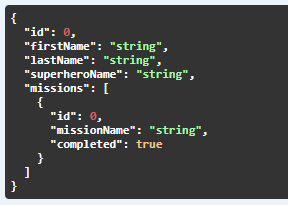
\includegraphics{./images/chapter-jpa/superhero_detail_dto}




